   \section{Introduction}
   
   \subsection{What is JOD?}
   
   JOD is a code, test and documentation \emph{refactoring} \href{http://www.jsoftware.com/jwiki/Addons}{\emph{Addon}}\index{Addon} for the
     \href{http://www.jsoftware.com}{\emph{J programming language}} \cite{RKWHui:jdictionary}. JOD has been 
      programmed entirely in J\footnote{JOD makes a few OS calls to move files and generate \texttt{GUIDs}.}
      and can be quickly ported to any system that supports J.
   
   \subsection{Why JOD?}  
   
   Programming in J 
   has a charming and distinctive flavor.  Tasks decompose into scores of tiny
   programs that are called \emph{words}. JOD stores and organizes
   J words and other objects in a dictionary database: hence the 
   name \textbf{J} \textbf{O}bject \textbf{D}ictionary.
   
   Code  databases are not new.  Similar systems have 
   been developed for many programming
   environments. Storing code in a database might strike you as obtuse.  
   Why compromise the ease, portability, and broad support of standard source code  
   files? Believe me,
   there are good reasons.
   
\begin{itemize}
	\item J encourages brevity: microscopic programs, words, accumulate rapidly.  
	\emph{Short J words are often general purpose words. } They can be used in many contexts.  How  
	are scores of terse words best employed? Scattering them in many scripts leads
	to error prone \emph{copy-and-pasting} or 
	 \emph{rampant over-inclusion}.\footnote{Over-inclusion occurs when you load 
	an entire class and only use a tiny portion of it.  Unused code is not harmless. It always confuses programmers.}  
	 The best way to reuse short words is to put
	 them in a system like JOD and fetch as required.   
	\item With JOD there is only \emph{one definition} for a given word. When word copies are
	 found in many files it's not always easy to find the current version.
	\item With JOD there are no significant limits on vocabulary size.  Scripts \emph{can} hold thousands
	of words but it's a nuisance to maintain and include such large files.
	\item The \emph{complete definition} of a word can 
	be quickly examined.  Good English dictionaries contain far more than
	definitions.  There are etymologies, synonyms, usage comments and illustrations.  Similarly,
	\emph{literate} software documentation contains far more than source code.  You will find
	descriptions of basic algorithms, remarks about coding techniques, references to
	published material, program test suites,\index{test suite} detailed error
	logs and germane diagrams. Storing such material in source code would 
	horribly clutter programs.  A dictionary is where this material belongs.
	\item \emph{Relationships between words} can be stored.  Accurate word references
	 make it easier to understand code.  This is especially true if references 
	  and documentation are linked. 
	\item JOD facilitates the \emph{generation of scripts and the distribution} of code. When I
	program with JOD I rarely write \texttt{load} scripts.  I use JOD to generate and distribute
  J scripts.  JOD can fetch and execute arbitrary J scripts so you can manage
  very elaborate generation and distribution procedures.
   \item Finally, \emph{JOD encourages a different way to think about programming.} When programs are
   reduced to their primary reusable units, words in J's case, many traditional software engineering problems
   almost disappear. With JOD code reuse and refactoring is fluid, natural and darn near unavoidable.
\end{itemize}

\section{Installing and Configuring JOD}\label{ss:jodcfgdesc}

Before using JOD you need to install the current Windows, Linux or Mac version of J.\footnote{JOD runs on 
 J \texttt{6.0x} ,  J \texttt{7.0x}  and J \texttt{8.0x} Windows systems. The Linux and Mac versions of JOD require J
\texttt{7.0x} or \texttt{8.0x}. Currently there are no \texttt{IOS} or \texttt{Android} versions of JOD. Porting JOD 
to any J system is a simple task.
If you are interested in helping me create ports please contact me at:  
\texttt{bakerjd99@gmail.com}
} J can be downloaded from \href{http://www.jsoftware.com}{\texttt{www.jsoftware.com}}.

In addition to J you need to install a number of J \emph{addons}. JOD uses the
\texttt{jfiles}, \texttt{regex} and \texttt{task} addons.  Some J versions
include these addons as part of the basic J system. If you can run the following J command
without errors your system is ready for JOD. 
\begin{lstlisting}[frame=single,framerule=0pt,label=lst:reqaddons]
   require 'jfiles regex task'
\end{lstlisting}
If you encounter any errors  use \href{http://www.jsoftware.com/jwiki/JAL/}{\texttt{JAL}}\index{installation!JAL} to install 
missing addons.
 
JOD can be installed in two ways.  
\begin{enumerate}
	\item Use \href{http://www.jsoftware.com/jwiki/Addons/general/jod}{\texttt{JAL}}\index{installation!JAL}, J's package manager 
	\cite{jwiki:jal}, to download JOD. \emph{Using JAL is the easiest way to install and maintain JOD.}
	\item Download the current JOD distribution from \href{http://bakerjd99.wordpress.com/the-jod-page/}{\emph{The JOD Page}}\index{installation!\emph{The JOD Page}} \cite{baker:jodpages} and unzip, preserving directories, to the relative directory\footnote{Paths that begin with the \textbf{\texttt{\~}} character are relative directories. The full path can be obtained with \texttt{jpath} verb. } \verb|~addons/general/jod|
\end{enumerate}

After installation JOD can be loaded with:\footnote{\textcolor{red}{The \texttt{'} character 
is a single quote: in J notation it is: \texttt{39 \{ a.}}
}
\begin{lstlisting}[frame=single,framerule=0pt,label=lst:loadjod00]
   load 'general/jod'
\end{lstlisting}

To configure and maintain JOD you must be aware of the following:
\begin{enumerate}
	\item JOD uses the J startup file \verb|~config/startup.ijs| to store load scripts: see 
	\hyperlink{il:mls}{\texttt{mls}} on page~\pageref{ss:mls}.  Exercise caution when manually
	editing JOD's load script section.
	\item To run JOD \href{http://www.jsoftware.com/help/user/lab_system_overview.htm}{labs}\index{labs} you must download and install the\index{Addon}
	 \href{http://www.jsoftware.com/jwiki/Addons/general/jodsource}{\texttt{jodsource}} addon \cite{baker:jodsource}. 
	 \texttt{jodsource} can be installed with \texttt{JAL}.
	\item JOD labs and test scripts assume some J folders have been configured.  Open J's
	configuration tool\index{configuration!tool}, see Figure~\ref{eps:jodfolders} on 
   page~\pageref{eps:jodfolders}, and
	define folders like:\index{configuration!J folders}
	\begin{lstlisting}[frame=single,framerule=0pt,label=lst:foldercfg]
   JOD               c:/jod
   JODDUMPS          c:/jod/joddumps
   JODSOURCE         c:/jodtest/labtesting
   JODTEST           c:/jodtest/test
  \end{lstlisting}
  \emph{Use fully qualified directory paths that are not in the J install tree.}
  \item \hyperlink{il:jodhelp}{\texttt{jodhelp}} (\pageref{ss:jodhelp}) uses a 
  PDF reader to display JOD documentation. Use J's configuration tool to set 
  your preferred PDF reader.\footnote{See the blog post \href{https://bakerjd99.wordpress.com/2015/03/22/jod-update-version-0-9-97/}{JOD Update: Version \texttt{0.9.97*}} for J configuration advice.
  } 
\end{enumerate} 


 % following figure is from bit map screen capture - I'm not thrilled at how it scales here
 % bit map inclusions have to be carefully matched to the output resolution of
 % of the display to give the best results.
% \begin{figure}[htbp]
%  \centering
%  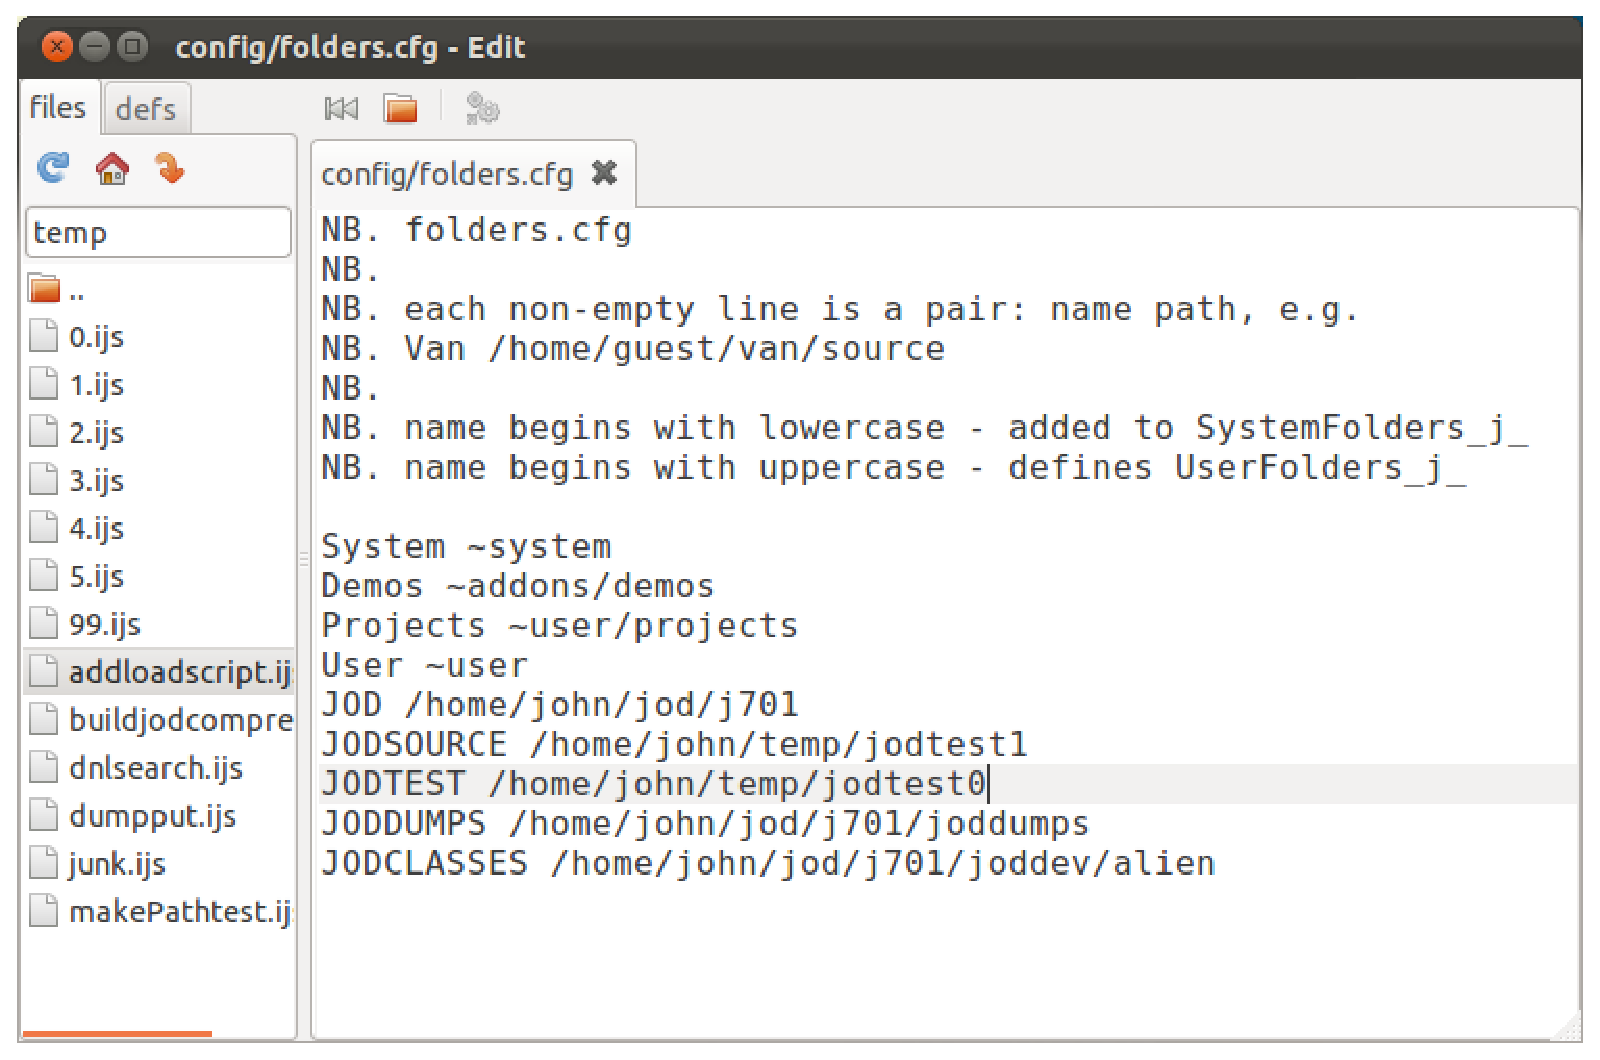
\includegraphics[width=\textwidth]{j7folders}
%  %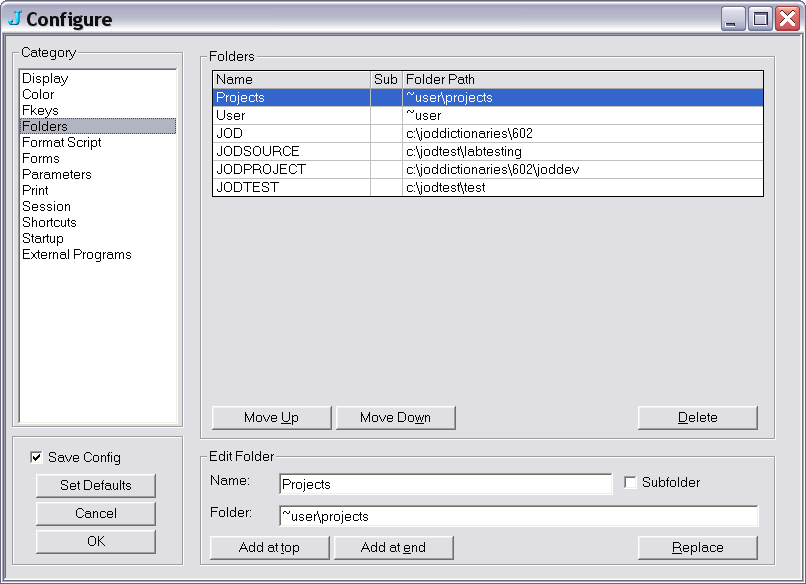
\includegraphics[width=\textwidth]{jodfolderconfig}
%  \caption[JOD Folders]{The following folder configuration\index{configuration!J folders} is recommended for running JOD labs and test scripts.  When defining JOD folders the full path, including the drive letter on Windows and a
%leading / for Linux, must be used.  The J configure utility does not reliably handle relative paths for directories outside of J's install tree. }
%   \label{eps:jodfolders}
%   \end{figure}

\begin{figure}[htbp]
  \centering
  \subfigure[J \texttt{8.0x} Windows JQT configuration editor]{
    \label{eps:j8folders}
    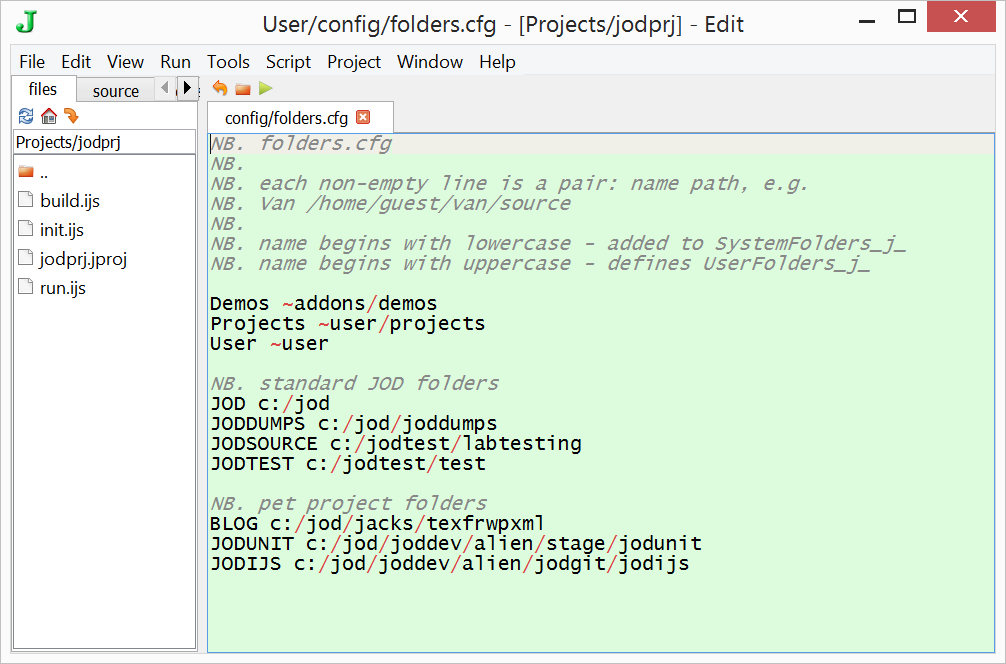
\includegraphics[width=0.8\textwidth]{j8folders}}
  \hfill
  \subfigure[J \texttt{8.0x} Mac JQT configuration editor]{
    \label{eps:j7folders}
    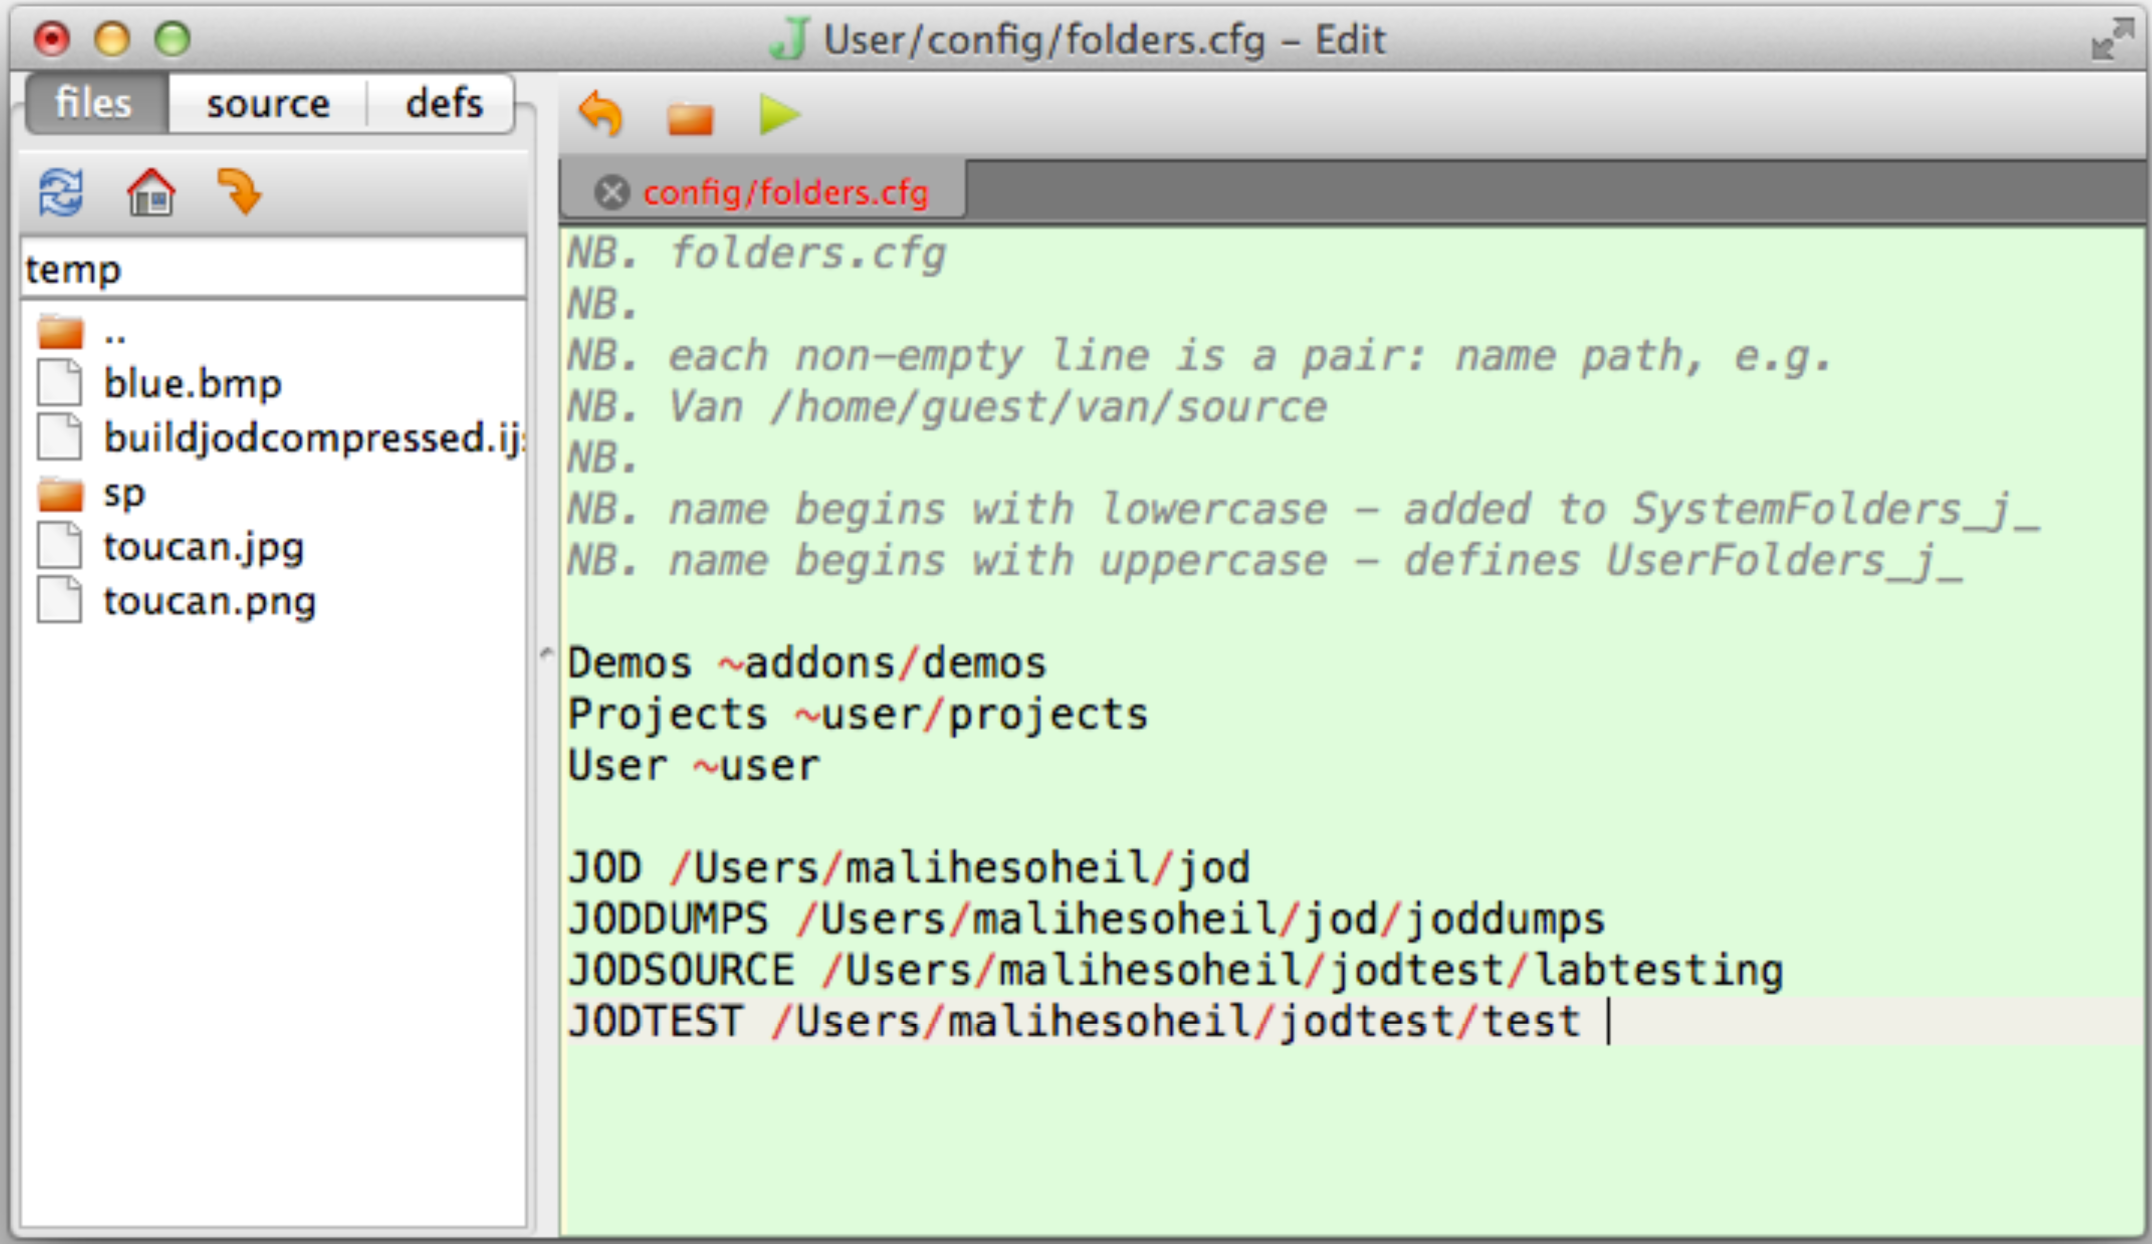
\includegraphics[width=0.7\textwidth]{mac32jqtcfg}}
\caption[JOD Folders]{This folder configuration\index{configuration!J folders} is recommended for 
running JOD labs and test scripts. 
When defining JOD folders the full path, including the drive letter on Windows and a
leading / for Linux and the Mac must be used: see page~\pageref{lst:foldercfg}.} 
  \label{eps:jodfolders}
\end{figure}
